%DIF 1c1-2
%DIF LATEXDIFF DIFFERENCE FILE
%DIF DEL first-draft.tex   Mon Apr 20 01:15:17 2020
%DIF ADD proposal.tex      Fri Apr 24 14:22:30 2020
%DIF < \documentclass[12pt, final]{article}
%DIF -------
\documentclass[11pt, final]{article} %DIF > 
\usepackage{mathpartir} %DIF > 
%DIF -------
\usepackage{stmaryrd}
\usepackage{mathtools}
\usepackage{array,booktabs,ragged2e}
\usepackage[english]{babel}
\usepackage[utf8]{inputenc}
\usepackage{graphicx}
\usepackage{fancyhdr}
\usepackage{amsthm}
\usepackage{microtype}
\usepackage[draft=false,cache]{minted}
\setlength{\marginparwidth}{3cm}
\usepackage[obeyFinal]{todonotes}
\usepackage{libertine}
% \usepackage{libertinust1math}
\usepackage{amsmath}
\usepackage[justification=centering]{caption}
\usepackage{csquotes}
%DIF 19a20
\usepackage{etoolbox} %DIF > 
%DIF -------
\usepackage{showkeys}
\usepackage[
  backend=biber,
  bibstyle=ieee,
  citestyle=ieee,
  sorting=ynt,
  hyperref=true,
  backref=true
]{biblatex}
% \usepackage[hidelinks]{hyperref}
%DIF 29c31
%DIF < \usepackage{hyperref}
%DIF -------
\usepackage[hidelinks]{hyperref} %DIF > 
%DIF -------
\usepackage{fontspec}
\setmainfont{TeX Gyre Pagella}
\setsansfont{TeX Gyre Heros}[Scale=MatchLowercase]
\setmonofont{Inconsolata}[Scale=MatchLowercase]
\RecustomVerbatimEnvironment{Verbatim}{BVerbatim}{}
\renewcommand{\figurename}{Listing}
\setminted[coq]{escapeinside=~~,mathescape}
%DIF 37a39-61
\newcommand{\br}[1]{\langle #1 \rangle} %DIF > 
\def\Yields{\Downarrow} %DIF > 
\newcommand{\makefootnotelist}[1]{% %DIF > 
    \parbox{0.8\textwidth} {% %DIF > 
        \footnotesize{% %DIF > 
            \renewcommand*{\do}[1]{##1\\}% %DIF > 
            \dolistcsloop{#1}}}}% %DIF > 
\newcommand{\fancyfootnote}[1]{% %DIF > 
    \footnotemark{}% %DIF > 
    \def\listname{footlist\thepage}% %DIF > 
    \def\n{$^{\the\numexpr\value{footnote}}$} %DIF > 
    \ifcsdef{\listname}% %DIF > 
        {\listcseadd{\listname}{\n\ #1}}% %DIF > 
        {\csedef{\listname}{}% %DIF > 
        \listcseadd{\listname}{\n\ #1}}% %DIF > 
    \fancypagestyle{fancyfootnote}{% %DIF > 
        \fancyfoot[L]{\makefootnotelist{\listname}}% %DIF > 
        \fancyfoot[C]{}% %DIF > 
        \fancyfoot[R]{\thepage}% %DIF > 
    }\thispagestyle{fancyfootnote}}% %DIF > 
\fancypagestyle{plain}{% %DIF > 
  \fancyfoot[C]{\thepage} %DIF > 
} %DIF > 
%DIF -------

\addbibresource{references.bib}
\setlength{\headheight}{15pt}
\pagestyle{fancy}
\lhead{Utrecht University}
%DIF 42-43c67-68
%DIF < \cfoot{\thepage}
%DIF < \rfoot{Curtis Chin Jen Sem}
%DIF -------
\rfoot{\thepage} %DIF > 
\cfoot{ } %DIF > 
%DIF -------
\renewcommand{\headrulewidth}{0.5pt}
\renewcommand{\footrulewidth}{0.5pt}
\renewcommand{\listingscaption}{Code snippet}
%DIF 47a72
 %DIF > 
%DIF -------
\def\Vakar{V\'{a}k\'{a}r}
\def\<#1>{\csname keyword@@#1\endcsname}
\begingroup
\makeatletter
\def\do#1{\expandafter\doaux\expandafter{\keyword@style{#1}}{#1}}
\def\doaux#1#2{\global\@namedef{keyword@@#2}{#1}}
\def\keyword@style#1{\textbf{#1}}
\do{Coq}
\do{Agda}
\def\keyword@style#1{\texttt{#1}}
\do{bottom}
\do{Equations}
%DIF 59a85
\do{Coquelicot} %DIF > 
%DIF -------
\do{Program}
%DIF 60a87-89
\do{Set} %DIF > 
\do{Prop} %DIF > 
\do{Type} %DIF > 
%DIF -------
\do{return}
\do{simpl}
\do{Either}
\do{sb}
\do{Dsb}
\do{Reals}
\do{R}
\endgroup
%DIF PREAMBLE EXTENSION ADDED BY LATEXDIFF
%DIF UNDERLINE PREAMBLE %DIF PREAMBLE
\RequirePackage[normalem]{ulem} %DIF PREAMBLE
\RequirePackage{color}\definecolor{RED}{rgb}{1,0,0}\definecolor{BLUE}{rgb}{0,0,1} %DIF PREAMBLE
\providecommand{\DIFaddtex}[1]{{\protect\color{blue}\uwave{#1}}} %DIF PREAMBLE
\providecommand{\DIFdeltex}[1]{{\protect\color{red}\sout{#1}}}                      %DIF PREAMBLE
%DIF SAFE PREAMBLE %DIF PREAMBLE
\providecommand{\DIFaddbegin}{} %DIF PREAMBLE
\providecommand{\DIFaddend}{} %DIF PREAMBLE
\providecommand{\DIFdelbegin}{} %DIF PREAMBLE
\providecommand{\DIFdelend}{} %DIF PREAMBLE
\providecommand{\DIFmodbegin}{} %DIF PREAMBLE
\providecommand{\DIFmodend}{} %DIF PREAMBLE
%DIF FLOATSAFE PREAMBLE %DIF PREAMBLE
\providecommand{\DIFaddFL}[1]{\DIFadd{#1}} %DIF PREAMBLE
\providecommand{\DIFdelFL}[1]{\DIFdel{#1}} %DIF PREAMBLE
\providecommand{\DIFaddbeginFL}{} %DIF PREAMBLE
\providecommand{\DIFaddendFL}{} %DIF PREAMBLE
\providecommand{\DIFdelbeginFL}{} %DIF PREAMBLE
\providecommand{\DIFdelendFL}{} %DIF PREAMBLE
%DIF HYPERREF PREAMBLE %DIF PREAMBLE
\providecommand{\DIFadd}[1]{\texorpdfstring{\DIFaddtex{#1}}{#1}} %DIF PREAMBLE
\providecommand{\DIFdel}[1]{\texorpdfstring{\DIFdeltex{#1}}{}} %DIF PREAMBLE
\newcommand{\DIFscaledelfig}{0.5}
%DIF HIGHLIGHTGRAPHICS PREAMBLE %DIF PREAMBLE
\RequirePackage{settobox} %DIF PREAMBLE
\RequirePackage{letltxmacro} %DIF PREAMBLE
\newsavebox{\DIFdelgraphicsbox} %DIF PREAMBLE
\newlength{\DIFdelgraphicswidth} %DIF PREAMBLE
\newlength{\DIFdelgraphicsheight} %DIF PREAMBLE
% store original definition of \includegraphics %DIF PREAMBLE
\LetLtxMacro{\DIFOincludegraphics}{\includegraphics} %DIF PREAMBLE
\newcommand{\DIFaddincludegraphics}[2][]{{\color{blue}\fbox{\DIFOincludegraphics[#1]{#2}}}} %DIF PREAMBLE
\newcommand{\DIFdelincludegraphics}[2][]{% %DIF PREAMBLE
\sbox{\DIFdelgraphicsbox}{\DIFOincludegraphics[#1]{#2}}% %DIF PREAMBLE
\settoboxwidth{\DIFdelgraphicswidth}{\DIFdelgraphicsbox} %DIF PREAMBLE
\settoboxtotalheight{\DIFdelgraphicsheight}{\DIFdelgraphicsbox} %DIF PREAMBLE
\scalebox{\DIFscaledelfig}{% %DIF PREAMBLE
\parbox[b]{\DIFdelgraphicswidth}{\usebox{\DIFdelgraphicsbox}\\[-\baselineskip] \rule{\DIFdelgraphicswidth}{0em}}\llap{\resizebox{\DIFdelgraphicswidth}{\DIFdelgraphicsheight}{% %DIF PREAMBLE
\setlength{\unitlength}{\DIFdelgraphicswidth}% %DIF PREAMBLE
\begin{picture}(1,1)% %DIF PREAMBLE
\thicklines\linethickness{2pt} %DIF PREAMBLE
{\color[rgb]{1,0,0}\put(0,0){\framebox(1,1){}}}% %DIF PREAMBLE
{\color[rgb]{1,0,0}\put(0,0){\line( 1,1){1}}}% %DIF PREAMBLE
{\color[rgb]{1,0,0}\put(0,1){\line(1,-1){1}}}% %DIF PREAMBLE
\end{picture}% %DIF PREAMBLE
}\hspace*{3pt}}} %DIF PREAMBLE
} %DIF PREAMBLE
\LetLtxMacro{\DIFOaddbegin}{\DIFaddbegin} %DIF PREAMBLE
\LetLtxMacro{\DIFOaddend}{\DIFaddend} %DIF PREAMBLE
\LetLtxMacro{\DIFOdelbegin}{\DIFdelbegin} %DIF PREAMBLE
\LetLtxMacro{\DIFOdelend}{\DIFdelend} %DIF PREAMBLE
\DeclareRobustCommand{\DIFaddbegin}{\DIFOaddbegin \let\includegraphics\DIFaddincludegraphics} %DIF PREAMBLE
\DeclareRobustCommand{\DIFaddend}{\DIFOaddend \let\includegraphics\DIFOincludegraphics} %DIF PREAMBLE
\DeclareRobustCommand{\DIFdelbegin}{\DIFOdelbegin \let\includegraphics\DIFdelincludegraphics} %DIF PREAMBLE
\DeclareRobustCommand{\DIFdelend}{\DIFOaddend \let\includegraphics\DIFOincludegraphics} %DIF PREAMBLE
\LetLtxMacro{\DIFOaddbeginFL}{\DIFaddbeginFL} %DIF PREAMBLE
\LetLtxMacro{\DIFOaddendFL}{\DIFaddendFL} %DIF PREAMBLE
\LetLtxMacro{\DIFOdelbeginFL}{\DIFdelbeginFL} %DIF PREAMBLE
\LetLtxMacro{\DIFOdelendFL}{\DIFdelendFL} %DIF PREAMBLE
\DeclareRobustCommand{\DIFaddbeginFL}{\DIFOaddbeginFL \let\includegraphics\DIFaddincludegraphics} %DIF PREAMBLE
\DeclareRobustCommand{\DIFaddendFL}{\DIFOaddendFL \let\includegraphics\DIFOincludegraphics} %DIF PREAMBLE
\DeclareRobustCommand{\DIFdelbeginFL}{\DIFOdelbeginFL \let\includegraphics\DIFdelincludegraphics} %DIF PREAMBLE
\DeclareRobustCommand{\DIFdelendFL}{\DIFOaddendFL \let\includegraphics\DIFOincludegraphics} %DIF PREAMBLE
%DIF LISTINGS PREAMBLE %DIF PREAMBLE
\RequirePackage{listings} %DIF PREAMBLE
\RequirePackage{color} %DIF PREAMBLE
\lstdefinelanguage{DIFcode}{ %DIF PREAMBLE
%DIF DIFCODE_UNDERLINE %DIF PREAMBLE
  moredelim=[il][\color{red}\sout]{\%DIF\ <\ }, %DIF PREAMBLE
  moredelim=[il][\color{blue}\uwave]{\%DIF\ >\ } %DIF PREAMBLE
} %DIF PREAMBLE
\lstdefinestyle{DIFverbatimstyle}{ %DIF PREAMBLE
	language=DIFcode, %DIF PREAMBLE
	basicstyle=\ttfamily, %DIF PREAMBLE
	columns=fullflexible, %DIF PREAMBLE
	keepspaces=true %DIF PREAMBLE
} %DIF PREAMBLE
\lstnewenvironment{DIFverbatim}{\lstset{style=DIFverbatimstyle}}{} %DIF PREAMBLE
\lstnewenvironment{DIFverbatim*}{\lstset{style=DIFverbatimstyle,showspaces=true}}{} %DIF PREAMBLE
%DIF END PREAMBLE EXTENSION ADDED BY LATEXDIFF

\begin{document}

\begin{titlepage}
\pagenumbering{gobble}

\begin{figure}
   \begin{minipage}{0.48\textwidth}
   \begin{flushleft}
    %  \includegraphics[scale=0.5]{Images/UU_LOGO.png}
   \end{flushleft}
   \end{minipage}\hfill
   \begin{minipage}{0.48\textwidth}
   \begin{flushright}
    %  \includegraphics[scale=0.2]{Images/Logo.png}
   \end{flushright}
   \end{minipage}
\end{figure}

\thispagestyle{fancy}

\vspace{1in}

\center

\textsc{\large Master Thesis Proposal}

\vspace{0.5in}

\noindent\makebox[\linewidth]{\rule{\linewidth}{1.2pt}}
\textsc{\textbf{\large Formalized Proof of Automatic Differentiation in \<Coq>}}
\noindent\makebox[\linewidth]{\rule{\linewidth}{1.2pt}}

\vspace{0.5in}

\begin{minipage}{0.48\textwidth}
    \begin{flushleft}
        \textit{Student:} \\
        Curtis Chin Jen Sem \\
        % crtschin@gmail.com
    \end{flushleft}
\end{minipage}
\begin{minipage}{0.48\textwidth}
    \begin{flushright}
    \textit{Supervisors:} \\
    Mathijs \Vakar{} \\
    Wouter Swierstra \\
    % Email
    % \end{flushright}
    % \begin{flushright}
    % Email
    \end{flushright}
\end{minipage}

\vspace{2in}

\textbf{\large Department of Information and Computing Science} \\
\textit{Last updated: \today}

\end{titlepage}

\newpage

\pagenumbering{arabic}
\setcounter{page}{2}
\tableofcontents
\newpage

\section{Introduction}

AI and machine learning research has sparked a lot of new interest in recent times\DIFdelbegin \DIFdel{due to its many applications and ability to solve complex problems very quickly.
This is regularly done using a technique called automatic differentiation.
But programming inside current frameworks is very limited}\DIFdelend \DIFaddbegin \DIFadd{. It has been used in fields such as computer vision, natural language processing, and as opponents in various games such as chess and Go.
In machine learning and more specifically neural network research, researchers set up functions referred to as layers between the input and output data and through an algorithm called back propagation, try to optimize the network such that it learns how to solve the problem implied by the data.
Back propagation makes heavy use of automatic differentiation, but programming in an environment which allows for automatic differentiation can be limited.
}

\DIFadd{Frameworks such as Tangent}\fancyfootnote{https://github.com/google/tangent} \DIFadd{or autograd}\fancyfootnote{https://github.com/HIPS/autograd} \DIFadd{make use of source code transformations and operator overloading, which can restrict which high-level optimizations one is able to apply to generated code. Support for higher-order derivatives is also limited.
}

\DIFadd{Programming language research has a rich history with many well-known both high- }\DIFaddend and \DIFdelbegin \DIFdel{cumbersome. One possible solution is to create }\DIFdelend \DIFaddbegin \DIFadd{low-level optimization techniques such as partial evaluation and deforestation.
If instead of a framework, we were to have }\DIFaddend a programming language that \DIFdelbegin \DIFdel{facilitates defining differentiable functions.
This could have many benefits such as both applying many of the established high and low level optimizations known in programming languages research, ease defining functions for use in a gradient descent optimization through higher order functions and correctness through the use of a possible type system}\DIFdelend \DIFaddbegin \DIFadd{is able to facilitate automatic differentiation, we would be able to apply many of these techniques. Through the use of higher-order functions and type systems, we would also get additional benefits such as code-reusability and correctness}\DIFaddend .

\DIFdelbegin \DIFdel{We }\DIFdelend \DIFaddbegin \DIFadd{In this thesis, we will }\DIFaddend aim to formalize an extendable \DIFaddbegin \DIFadd{correctness }\DIFaddend proof of an implementation of automatic differentiation on a \DIFdelbegin \DIFdel{simply typed }\DIFdelend \DIFaddbegin \DIFadd{simply-typed }\DIFaddend lambda calculus in the \<Coq> proof assistant, opening up further possibilities for formally proving the correctness of more complex language features in the future.
Our formalization is based on a recent proof by \DIFdelbegin \DIFdel{Stanton Huot, }\DIFdelend \DIFaddbegin \DIFadd{Huot, Staton, }\DIFaddend and \Vakar{} \cite{huot2020correctness}.
They proved, using a denotational model of diffeological spaces, that their forward mode emulating macro is correct when applied to a \DIFdelbegin \DIFdel{simply typed }\DIFdelend \DIFaddbegin \DIFadd{simply-typed }\DIFaddend lambda calculus with products, co-products and inductive types.

\todo{Fill in}

With this thesis we will aim for the following goals:
\begin{itemize}
  \item \DIFdelbegin \DIFdel{Contribute a formalized proof of forward-mode automatic differentiation }\DIFdelend \DIFaddbegin \DIFadd{Formalize the proofs of both the forward mode and continuation-based automatic differentiation algorithms specified by Huot, Staton, and }\Vakar{} \DIFadd{\mbox{%DIFAUXCMD
\cite{huot2020correctness} }\hspace{0pt}%DIFAUXCMD
}\DIFaddend in \<Coq>.
  %DIF >  \item Formulate the proofs such that it facilitates further extensions.
  %DIF >  \item Extend the proof to polymorphic types.
  %DIF >  \item Adapt the proof to a small imperative language.
  \item \DIFdelbegin \DIFdel{Formulate the proofs such that it facilitates further extensions.
  }%DIFDELCMD < \item %%%
\item%DIFAUXCMD
\DIFdel{Extend the proof to polymorphic types.
  }%DIFDELCMD < \item %%%
\item%DIFAUXCMD
\DIFdel{Adapt the proof to a small imperative language.
  }%DIFDELCMD < \item %%%
\item%DIFAUXCMD
\DIFdelend Prove that well-known \DIFaddbegin \DIFadd{compile-time }\DIFaddend optimizations such as the partial evaluation, are correct with respect to \DIFaddbegin \DIFadd{the semantics of }\DIFaddend automatic differentiation.
  \item \DIFdelbegin \DIFdel{Prove the correctness of the continuation-based automatic differentiation algorithm. }\DIFdelend \DIFaddbegin \DIFadd{Extend the proof with the array types and compile-time optimization rules by Shaikhha, et. al.\mbox{%DIFAUXCMD
\cite{Shaikha2019}}\hspace{0pt}%DIFAUXCMD
.
  }\DIFaddend % \item (TODO: UNLIKELY) Extend the original proof with iteration and possibly recursion.
  % \item (TODO: MAYBE) Extend the original proof with inductive types.
  % \item (TODO: MAYBE) Extend the original proof with polymorphism.
  % \item (TODO: MAYBE) Adapt the proof to a small imperative language.
  % \item (TODO: LIKELY) Prove that well-known optimizations such as the partial evaluation, are correct with respect to automatic differentiation.
  % \item (TODO: LIKELY) Prove the correctness of the continuation-based automatic differentiation algorithm.
\end{itemize}

%DIF <  Ideally?:
%DIF <  Contributing an extendable proof of a simply typed lambda calculus
%DIF <  On which both the correctness of optimizations and language
%DIF <  extensions could be proven
%DIF <  Proof of optimizations maintaining correctness (partial evaluation)
\DIFdelbegin %DIFDELCMD < 

%DIFDELCMD < %%%
\DIFdelend As a notational convention, we will use specialized notation in the definitions themselves. Coq \DIFaddbegin \DIFadd{normally }\DIFaddend requires that pretty printed \DIFdelbegin \DIFdel{notation }\DIFdelend \DIFaddbegin \DIFadd{notations }\DIFaddend be defined separately from the definitions they reference. \DIFaddbegin \DIFadd{The letter $\Gamma$ is used for typing contexts while lowercase Greek letters are usually used for types.
}\DIFaddend 

\section{Background}

\subsection{Automatic differentiation}

% http://jmlr.org/papers/volume18/17-468/17-468.pdf

One of the principal techniques used in machine learning is back propagation, which calculates the gradient of a function. The \DIFdelbegin \DIFdel{idea being to use the gradient }\DIFdelend \DIFaddbegin \DIFadd{gradient itself is used }\DIFaddend in the gradient descent algorithm \DIFaddbegin \DIFadd{to optimize an objective functions by determining the direction of steepest descent}\DIFaddend \cite{Baydin2015AutomaticDI}.
Automatic differentiation has a long and rich history, where its \DIFdelbegin \DIFdel{main purpose is to }\DIFdelend \DIFaddbegin \DIFadd{driving motivation is to be able to }\DIFaddend automatically calculate the derivative of a function \DIFdelbegin \DIFdel{, or more precisely, calculate this derivative of a function described by a program }\DIFdelend \DIFaddbegin \DIFadd{in a manner that is both correct and fast.
Through techniques such as source-code transformations or operator overloading, one is able to implement an automatic differentiation algorithm which can transform any program which implements some function to one that calculates its derivative}\DIFaddend .
So in addition to the standard semantics present in most \DIFdelbegin \DIFdel{functional }\DIFdelend programming languages, \DIFdelbegin \DIFdel{we also now deal with relevant concepts }\DIFdelend \DIFaddbegin \DIFadd{concepts relevant to differentiation }\DIFaddend such as derivative values and the chain rule \DIFaddbegin \DIFadd{are needed}\DIFaddend .

Automatic or algorithmic differentiation is beneficial over other methods of automatically calculating the derivatives of functions such as numerical differentiation or symbolic differentiation due to its balance between speed and computational complexity.
There are two main \DIFdelbegin \DIFdel{modes }\DIFdelend \DIFaddbegin \DIFadd{variants }\DIFaddend of automatic differentiation\DIFdelbegin \DIFdel{.
These are namely forward }\DIFdelend \DIFaddbegin \DIFadd{, namely forward mode }\DIFaddend and reverse mode \DIFdelbegin \DIFdel{AD.
For the purposes of this paper, we will only discuss forward mode AD.
}\DIFdelend \DIFaddbegin \DIFadd{automatic differentiation.
}\DIFaddend 

In forward mode automatic differentiation \DIFaddbegin \DIFadd{every term in }\DIFaddend the function trace is \DIFdelbegin \DIFdel{accompanied with a dual numbers representation which calculate the derivative of the function}\DIFdelend \DIFaddbegin \DIFadd{annotated with the corresponding derivative of that term}\DIFaddend . These are also known as the respectively the primal and tangent traces. So every partial derivative of every \DIFdelbegin \DIFdel{sub function }\DIFdelend \DIFaddbegin \DIFadd{sub-function }\DIFaddend is calculated parallel to its counterpart. We will take the function $f(x, y) = x^2 + (x - y)$ as an example. The dependencies between the terms and operations of the function is visible in the computational graph in \DIFdelbegin \DIFdel{figure}\DIFdelend \DIFaddbegin \DIFadd{Figure}\DIFaddend ~\ref{fig:func_trace}. The corresponding traces are filled in \DIFdelbegin \DIFdel{table}\DIFdelend \DIFaddbegin \DIFadd{Table}\DIFaddend ~\ref{table:func_trace} for the input values $x = 2, y = 1$. We can calculate the partial derivative $\frac{\delta f}{\delta x}$ at this point by setting $x' = 1$ and $y' = 0$. In this paper we will prove the correctness of a simple forward mode automatic differentiation algorithm with respect to the semantics of a \DIFdelbegin \DIFdel{simply typed }\DIFdelend \DIFaddbegin \DIFadd{simply-typed }\DIFaddend lambda calculus.

\DIFdelbegin %DIFDELCMD < \begin{figure}[h]
%DIFDELCMD <   %%%
\DIFdelendFL \DIFaddbeginFL \DIFaddFL{Reverse mode automatic differentiation takes a different approach. It tries to work backwards from the output by annotating each intermediate variable $v_i$ with an adjoint $v'_i=\frac{\delta y_i}{\delta v_i}$. To do this, two passes are necessary. Like the forward mode variant the primal trace is needed to determine the intermediate variables and function dependencies. These are recorded in the first pass. The second pass actually calculates the derivatives by working backwards from the output using the adjoints, also called the adjoint trace.
}

\DIFaddFL{The choice between automatic differentiation variant is heavily dependent on the function being differentiated. The number of applications of the forward mode algorithm is dependent on the number of input variables, as it has to be redone for each possible partial derivative of the function. On the other hand, reverse mode AD has to work backwards from each output variable. In machine learning research, reverse mode AD is generally preferred as the objective functions regularly contain a very small number of output variables. How one does reverse mode automatic differentiation on a functional language is still an active area of research. Huot, Staton and }\Vakar{} \DIFaddFL{have proposed a continuation-based algorithm which mimic much of the same ideas as reverse mode automatic differentiation\mbox{%DIFAUXCMD
\cite{huot2020correctness}}\hspace{0pt}%DIFAUXCMD
.
}

\begin{figure}
  \DIFaddendFL \centering
  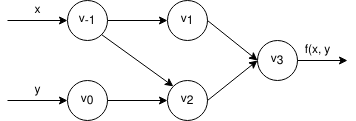
\includegraphics[scale=0.6]{assets/function_trace.png}
  \caption{Computational graph of $f(x, y) = x^2 + (x - y)$}
  \label{fig:func_trace}
\end{figure}

\DIFdelbegin %DIFDELCMD < \begin{figure}[h]
%DIFDELCMD <   %%%
\DIFdelendFL \DIFaddbeginFL \begin{table}
  \DIFaddendFL \begin{center}
    \begin{tabular}{ l l l l l | l l l l l }
      \hline
      \multicolumn{5}{l}{Primal trace} & \multicolumn{5}{l}{Tangent trace} \\
      \hline
$v_{-1} $&$=$&$x$&$=$&$2$             &$v'_{-1}$&$=$&$x'$&$=$&$1$ \\
$v_0    $&$=$&$y$&$=$&$1$             &$v'_{0}$&$=$&$y'$&$=$&$0$ \\
      \hline
$v_1    $&$=$&$v_{-1}^2$&$=$&$4$      &$v'_{1}$&$=$&$2*v_{-1}$&$=$&$4$ \\
$v_2    $&$=$&$v_{-1} - v_{0}$&$=$&$1$&$v'_{2}$&$=$&$v'_{-1}-v'_{0}$&$=$&$1$ \\
$v_3    $&$=$&$v_1 + v_2$&$=$&$5$     &$v'_{3}$&$=$&$v'_1 + v'_2$&$=$&$5$ \\
      \hline
$f      $&$=$&$v_3$&$=$&$5$           &$f'$&$=$&$v'_3$&$=$&$5$ \\
      \hline
    \end{tabular}
  \end{center}
  \caption{Primal and tangent traces of $f(x, y) = x^2 + (x - y)$}
  \label{table:func_trace}
\DIFdelbeginFL %DIFDELCMD < \end{figure}
%DIFDELCMD < %%%
\DIFdelend \DIFaddbegin \end{table}
\DIFaddend 

\DIFdelbegin %DIFDELCMD < \todo{Fill in}
%DIFDELCMD < 

%DIFDELCMD < %%%
\DIFdelend \subsection{Denotational semantics}
% A formal semantics of programming language: An introduction

The notion of denotational semantics tries to find underlying mathematical models able to underpin the concepts known in programming languages. The most well-known example is the solution given by Dana Scott and Christopher Strachey\cite{Scott1977} for lambda calculi, also called domain theory.
To be able to formalize non-termination and partiality, they thought to use concepts such as partial orderings and least fixed points\cite{aaby2020}.
In this model, programs are interpreted as partial functions\DIFdelbegin \DIFdel{and }\DIFdelend \DIFaddbegin \DIFadd{, and recursive }\DIFaddend computations as taking the fixpoint of such functions.
Non-termination, on the other hand, is formalized as a value \<bottom> that is lower in the ordering relation than any other element.

In our specific case, we try to find a satisfactory model we can use to show that our implementation of forward mode automatic differentiation is correct when applied to a \DIFdelbegin \DIFdel{simply typed }\DIFdelend \DIFaddbegin \DIFadd{simply-typed }\DIFaddend lambda calculus.
In the original pen and paper proof of automatic differentiation this thesis is based on, the mathematical models used were diffeological spaces, which are \DIFaddbegin \DIFadd{a }\DIFaddend generalization of smooth manifolds.
For the purpose of this thesis, however, \DIFdelbegin \DIFdel{this was deemed excessive and much too difficult and time consuming to implement in a mathematically sound manner in }\DIFdelend \DIFaddbegin \DIFadd{we were able to avoid using diffeological spaces as recursion, iteration and concepts dealing with non-termination and partiality are left out of the scope of this thesis.
}\DIFaddend \<Coq> \DIFaddbegin \DIFadd{has very limited support for domain theoretical models.
There are possible libraries which have resulted from experiments trying to encode domain theoretical models\mbox{%DIFAUXCMD
\cite{Benton2009}}\hspace{0pt}%DIFAUXCMD
\mbox{%DIFAUXCMD
\cite{Dockins2014}}\hspace{0pt}%DIFAUXCMD
, but these are incompatible with recent versions of \<Coq>}\DIFaddend .
As \DIFdelbegin \DIFdel{such, we chose to make use of }\DIFdelend \DIFaddbegin \DIFadd{a part of its type system, }\DIFaddend \<Coq> \DIFdelbegin \DIFdel{'s existing types as denotations and base the relation on the denotations instead of the syntactic structures. Due to }\DIFdelend \DIFaddbegin \DIFadd{contains a set-theoretical model available under the sort \<Set>, which is satisfactory as }\DIFaddend the \DIFdelbegin \DIFdel{relative simplicity of the language, we did not yet require domain theoretical concepts. If recursion or iteration were to be added to the language, it is currently expected that these would be needed}\DIFdelend \DIFaddbegin \DIFadd{denotational semantics for our language.
}

\DIFadd{Because we use the real numbers as the ground type in our language, we also needed an encoding of the real numbers in Coq. The library for real numbers in \<Coq> has improved in recent times from one based on a completely axiomatic definition to one involving Cauchy sequences}\fancyfootnote{https://coq.inria.fr/library/Coq.Reals.ConstructiveCauchyReals.html}\DIFadd{. For the purposes of this thesis, however, we needed differentiability as the denotational result of applying the macro operation. Instead of encoding this by hand, we opted for the more comprehensive library \<Coquelicot>\mbox{%DIFAUXCMD
\cite{Boldo2015CoquelicotAU}}\hspace{0pt}%DIFAUXCMD
, which contains many general definitions for differentiating functions}\DIFaddend .

\todo{Fill in}

\subsection{Coq}

\<Coq> is a proof assistant \DIFdelbegin \DIFdel{created by Thierry Coquand as an implementation of his }\DIFdelend \DIFaddbegin \DIFadd{based on the }\DIFaddend calculus of constructions type theory \DIFaddbegin \DIFadd{created by Thierry Coquand and G\'{e}rard Huet}\DIFaddend \cite{Coquand1988}.
In the 30 years since it has been released, research has contributed to extending the proof assistant with additional features such as inductive and co-inductive data types\cite{Coquand1990}, dependent pattern matching\cite{Sozeau2010} and advanced modular constructions for organizing \DIFdelbegin \DIFdel{colossal }\DIFdelend \DIFaddbegin \DIFadd{large }\DIFaddend mathematical proofs\cite{Sozeau2008}\cite{Mahboubi2013}.

The core of this type theory is based on constructive logic and so many of the laws known in classical logic are not \DIFdelbegin \DIFdel{present.
Examples include }\DIFdelend \DIFaddbegin \DIFadd{provable.
An example includes }\DIFaddend the law of the excluded middle, $\forall A, A \vee \neg A$\DIFdelbegin \DIFdel{, or the law of functional extensionality, $(\forall x, f(x) = g(x)) \rightarrow f = g$.
In most }\DIFdelend \DIFaddbegin \DIFadd{.
In some }\DIFaddend cases they can, however, be safely added to \<Coq> without making its logic inconsistent. \DIFaddbegin \DIFadd{These are readily available in the standard library.
}\DIFaddend Due to its usefulness in proving propositions over functions, we will make use of the functional extensionality axiom in \<Coq>.

\subsubsection{Language representation}
\label{sec:language_repr}

\DIFaddbegin \begin{figure}
  \begin{mathpar}
    \inferrule*[Right=\textsc{TVar}]
      {\DIFaddFL{elem\ n\ \Gamma = \tau}}
      {\DIFaddFL{\Gamma \vdash var\ n : \tau}} \and
    \inferrule*[Right=\textsc{TAbs}]
      {\DIFaddFL{(\sigma, \Gamma) \vdash t : \tau}}
      {\DIFaddFL{\Gamma \vdash t : \sigma \rightarrow \tau}} \\ \and
    \inferrule*[Right=\textsc{TApp}]
      {\DIFaddFL{\Gamma \vdash t1 : \sigma \rightarrow \tau }\\
        \DIFaddFL{\Gamma \vdash t2 : \sigma}}
      {\DIFaddFL{\Gamma \vdash t1\ t2 : \tau}}
  \end{mathpar}
  \label{fig:stlc_infer}
  \caption{\DIFaddFL{Type-inferrence rules for a simply-typed lambda calculus using De-Bruijn indices}}
\end{figure}

\DIFaddend When defining a \DIFdelbegin \DIFdel{simply typed }\DIFdelend \DIFaddbegin \DIFadd{simply-typed }\DIFaddend lambda calculus, there are two main possibilities\cite{plfa2019}.
The arguably simpler variant, known as an extrinsic representation, is traditionally the one introduced to new students learning \<Coq>.
In the \DIFdelbegin \DIFdel{extensional }\DIFdelend \DIFaddbegin \DIFadd{extrinsic }\DIFaddend representation, the terms themselves are untyped and typing judgments are defined separately as relations between the types and terms. A basic example of working with this is given in \DIFaddbegin \DIFadd{Software Foundations}\DIFaddend \cite{Pierce:SF2}.
This, however, required many additional lemmas and machinery to be proved \DIFdelbegin \DIFdel{.
}\DIFdelend \DIFaddbegin \DIFadd{to be able to work with both substitutions and contexts as these are defined separate from the terms.
As an example, the preservation property which states that reduction does not change the type of a term, needs to be proven explicitly.
}\DIFaddend The other approach, also called an intrinsic representation, makes use of just a single well-typed definition.
Ill-typed terms are made impossible by the type checker.
This representation, while beneficial in the proof load, however complicates much of the normal machinery involved in programming language theory.
One example is how one would define operations such as substitutions \DIFaddbegin \DIFadd{or weakening}\DIFaddend .

But even when choosing an intrinsic representation, the problem of variable binding persists.
Much meta-theoretical research has been done on possible approaches to this problem each with their own advantages and disadvantages.
The POPLmark challenge gives a comprehensive overview of each of the possibilities in various proof assistants\cite{Aydemir2005}.
An example of an approach is the nominal representation where every variable is named.
While this does follow the standard format used in regular mathematics, problems such as alpha-conversion and capture-avoidance \DIFdelbegin \DIFdel{arise}\DIFdelend \DIFaddbegin \DIFadd{appears}\DIFaddend .

\begin{listing}[h]
  \begin{minted}{coq}
  Inductive ty : Type :=
    | ~unit~ : ~ty~
    | ~\Rightarrow~ : ~ty \rightarrow ty \rightarrow ty~.

  Inductive tm : Type :=
    | var : ~string \rightarrow tm ~
    | abs : ~string \rightarrow ty \rightarrow tm \rightarrow tm~
    | app : ~tm \rightarrow tm \rightarrow tm~.
  \end{minted}
  \caption{Simply typed \lambda-calculus using an extrinsic nominal representation.}
  \label{lst:nominal_stlc}
\end{listing}

The approach used in the rest of this thesis is an extension of the \DIFdelbegin \DIFdel{de-bruijn }\DIFdelend \DIFaddbegin \DIFadd{De-Bruijn }\DIFaddend representation which numbers variables relative to the binding lambda term.
In this representation the variables are referred to as \DIFdelbegin \DIFdel{de-bruijn }\DIFdelend \DIFaddbegin \DIFadd{well-typed De-Bruijn }\DIFaddend indices.
A significant benefit of this representation is that the problems of capture avoidance and alpha equivalence are avoided.
As an \DIFdelbegin \DIFdel{alteration}\DIFdelend \DIFaddbegin \DIFadd{alternative}\DIFaddend , instead of using numbers to represent the distance, indices within the typing context can be used to ensure that a variable is always well-typed and well-scoped.
\DIFdelbegin \DIFdel{The }\DIFdelend \DIFaddbegin \DIFadd{While the idea of using type indexed terms has been both described and used by many authors\mbox{%DIFAUXCMD
\cite{Altenkirch99}}\hspace{0pt}%DIFAUXCMD
\mbox{%DIFAUXCMD
\cite{McBride04}}\hspace{0pt}%DIFAUXCMD
\mbox{%DIFAUXCMD
\cite{Adams06}}\hspace{0pt}%DIFAUXCMD
, the }\DIFaddend specific formulation used in this thesis \DIFaddbegin \DIFadd{using both substitutions and rename operations }\DIFaddend was fleshed out \DIFaddbegin \DIFadd{in Coq }\DIFaddend by Nick Benton, et. al.\DIFdelbegin \DIFdel{in }\DIFdelend \cite{Benton2011}, and was also used as one of the examples in the second POPLmark challenge which deals with logical relations\cite{poplmark_reloaded}.
While this does \DIFdelbegin \DIFdel{subvert }\DIFdelend \DIFaddbegin \DIFadd{avoid }\DIFaddend the problems present in the nominal representation, it unfortunately does have some problems of its own.
Variable substitutions have to be defined using two separate renaming and substitution operations.
Renaming is formulated as extending the typing context of variables, while substitution actually swaps the variables for terms.
Due to using indices from the context as variables, some lifting boilerplate is also needed to manipulate contexts.

\begin{listing}[h]
  \begin{minted}{coq}
  Inductive ~\tau \in \Gamma~ : Type :=
    | Top : ~\forall \Gamma \tau, \tau \in (\tau::\Gamma)~
    | Pop : ~\forall \Gamma \tau \sigma, \tau \in \Gamma \rightarrow \tau \in (\sigma::\Gamma)~.

  Inductive tm ~\Gamma \tau~ : Type :=
    | var : ~\forall \Gamma \tau, \tau \in \Gamma \rightarrow tm \Gamma \tau~
    | abs : ~\forall \Gamma \tau \sigma, tm (\sigma::\Gamma) \tau \rightarrow tm \Gamma (\sigma \Rightarrow \tau)~
    | app : ~\forall \Gamma \tau \sigma, tm \Gamma (\sigma \Rightarrow \tau) \rightarrow tm \Gamma \sigma \rightarrow tm \Gamma \tau~.
  \end{minted}
  \caption{Basis of a \DIFdelbegin \DIFdel{simply typed }\DIFdelend \DIFaddbegin \DIFadd{simply-typed }\DIFaddend \lambda-calculus using a strongly typed intrinsic formulation.}
  \label{lst:strong_stlc}
\end{listing}
\todo{Extend example}

\subsubsection{\DIFdelbegin \DIFdel{Dependent }\DIFdelend \DIFaddbegin \DIFadd{Dependently-typed }\DIFaddend programming in Coq}

In \<Coq>, one can normally write function definitions using either case-analysis as is done in other functional languages, or using \<Coq>'s tactics.
If proof terms are present in the function definition, however, it is customary to write it using tactics because of the otherwise \DIFdelbegin \DIFdel{cumbersome }\DIFdelend \DIFaddbegin \DIFadd{complicated }\DIFaddend and verbose code \DIFdelbegin \DIFdel{needed to pattern-match on the arguments.
But this can be troublesome in the cases where }\DIFdelend \DIFaddbegin \DIFadd{due to }\DIFaddend the \DIFaddbegin \DIFadd{previously poor support for dependent pattern matching in Coq.
But if the functionality is not immediately apparent from the }\DIFaddend function signature\DIFdelbegin \DIFdel{is ambiguous, as }\DIFdelend \DIFaddbegin \DIFadd{, }\DIFaddend it can be hard to recognize what the function then \DIFdelbegin \DIFdel{actually }\DIFdelend computes.
One other possibility would be to write the function \DIFdelbegin \DIFdel{using relations }\DIFdelend \DIFaddbegin \DIFadd{as a relation }\DIFaddend between its input and output.
This also has its limitations as \DIFdelbegin \DIFdel{relations can be tricky to define}\DIFdelend \DIFaddbegin \DIFadd{you then lose computability as Coq treats these definitions opaquely}\DIFaddend . In this case \DIFdelbegin \DIFdel{, the definitions are also opaque such that the }\DIFdelend \DIFaddbegin \DIFadd{the }\DIFaddend standard \<simpl> tactic which invokes \<Coq>'s reduction mechanism is not able to reduce \DIFaddbegin \DIFadd{instances of }\DIFaddend the term.
This often requires the user to write \DIFdelbegin \DIFdel{to write }\DIFdelend many more proofs to be able to work with the definitions.

As an example, we will work through defining a length indexed list and a corresponding head function, which is well known to be partial.
Using the \<Coq> keyword return, it is possible to let the return type of a match expression depend on the result of one of the type arguments.
This makes it possible to specify what the return type of the empty list should be.
In \DIFdelbegin \DIFdel{snippet}\DIFdelend \DIFaddbegin \DIFadd{Snippet}\DIFaddend ~\ref{lst:dt_ilist}, we use the unit type which contains just one inhabitant, \<tt>.

\begin{listing}
  \begin{minted}{coq}
  Inductive ilist : ~Type \rightarrow nat \rightarrow Type~ :=
    | nil : ~\forall A, ilist A 0~
    | cons : ~\forall A n, A \rightarrow ilist A n \rightarrow ilist A (S n)~

  Definition hd {A} n (ls : ilist A n) :=
    match ls in (ilist A n) return
      (match n with
      | O => unit
      | S _ => A end) with
    | nil => tt
    | cons h _ => h
  end.
  \end{minted}
  \caption{Definition of a length indexed list and hd using the return keyword, adapted from \DIFaddbegin \DIFadd{Certified Programming with Dependent Types}\DIFaddend \cite{ChlipalaCPDT}.}
  \label{lst:dt_ilist}
\end{listing}

\DIFdelbegin \DIFdel{In \mbox{%DIFAUXCMD
\cite{Sozeau2006} }\hspace{0pt}%DIFAUXCMD
and \mbox{%DIFAUXCMD
\cite{Sozeau2007} }\hspace{0pt}%DIFAUXCMD
}\DIFdelend \DIFaddbegin \DIFadd{Mathieu }\DIFaddend Sozeau introduces an extension to \<Coq> via a new keyword \<Program> which allows the use of case-analysis in more complex definitions\DIFaddbegin \DIFadd{\mbox{%DIFAUXCMD
\cite{Sozeau2006}}\hspace{0pt}%DIFAUXCMD
\mbox{%DIFAUXCMD
\cite{Sozeau2007}}\hspace{0pt}%DIFAUXCMD
}\DIFaddend .
To be more specific, it allows definitions to be specified separately from \DIFdelbegin \DIFdel{its }\DIFdelend \DIFaddbegin \DIFadd{their }\DIFaddend accompanying proofs, possibly filling them in automatically if possible.
While this does improve on the previous situation, using the definitions in proofs can often be unwieldy due to the amount of boilerplate introduced.
This makes debugging error messages even harder than it already is in a proof assistant. This approach was used by Benton in his formulation of strongly typed terms.

Sozeau further improves on this \DIFdelbegin \DIFdel{in \mbox{%DIFAUXCMD
\cite{Sozeau2010} }\hspace{0pt}%DIFAUXCMD
and \mbox{%DIFAUXCMD
\cite{Sozeau2019} }\hspace{0pt}%DIFAUXCMD
by }\DIFdelend introducing a method for user-friendlier dependently-typed \DIFdelbegin \DIFdel{programming }\DIFdelend \DIFaddbegin \DIFadd{pattern matching }\DIFaddend in \<Coq> \DIFdelbegin \DIFdel{as the }\DIFdelend \DIFaddbegin \DIFadd{in the form of the }\DIFaddend \<Equations> library\DIFaddbegin \DIFadd{\mbox{%DIFAUXCMD
\cite{Sozeau2010}}\hspace{0pt}%DIFAUXCMD
\mbox{%DIFAUXCMD
\cite{Sozeau2019}}\hspace{0pt}%DIFAUXCMD
}\DIFaddend .
This introduces \<Agda>-like dependent pattern matching with with-clauses.
It does this by using a notion called coverings, where a covering is a set of equations such that the pattern matchings of the type signature are exhaustive.
There are two main ways to integrate this in a dependently typed environment, externally where it is integrated as high-level constructs in the pattern matching core as \<Agda> does it, or internally by using the existing type theory and finding witnesses of the covering to prove the definition correct, which is the approach used by Sozeau.
Due to the intrinsic typeful representation this paper uses, much of this was invaluable when defining the substitution operators as the regular type checker in Coq often had difficulty \DIFdelbegin \DIFdel{when recognizing type equalities }\DIFdelend \DIFaddbegin \DIFadd{type checking dependently typed terms }\DIFaddend in certain cases.

\begin{listing}
  \begin{minted}{coq}
  Equations hd {A n} (ls : ilist A n) (pf : n <> 0%nat) : A :=
  hd nil pf with pf eq_refl := {\DIFdelbegin \DIFdel{| x :=! x }\DIFdelend };
  hd (cons h n) _ := h.
  \end{minted}
  \caption{Definition of hd using \<Equations>}
  \label{lst:dt_ilist_hd_equations}
\end{listing}

\todo{Fill in}

\subsection{Logical relations}

Logical relations is \DIFaddbegin \DIFadd{a }\DIFaddend technique often employed when proving programming language properties \DIFaddbegin \DIFadd{of statically typed languages}\DIFaddend \cite{skorstengaard2019introduction}. There are two main ways they are used, namely as unary and binary relations.
Unary logical relations, also known as logical predicates, are predicates over single terms and are typically used to prove language characteristics such as type safety or strong normalization.
Binary logical relations on the other hand are used to prove program equivalences, usually in the context of denotational semantics as we will do.
\DIFaddbegin \DIFadd{There have been many variations on the versatile technique from syntactic step-indexed relations which have been used to solve recursive types\mbox{%DIFAUXCMD
\cite{Ahmed2006}}\hspace{0pt}%DIFAUXCMD
, to open relations which enable working with terms of non-ground type\mbox{%DIFAUXCMD
\cite{barthe2020versatility}}\hspace{0pt}%DIFAUXCMD
\mbox{%DIFAUXCMD
\cite{huot2020correctness}}\hspace{0pt}%DIFAUXCMD
.
}\DIFaddend Logical relations in essence are \DIFdelbegin \DIFdel{simply relations }\DIFdelend \DIFaddbegin \DIFadd{relations between terms }\DIFaddend defined by induction on \DIFdelbegin \DIFdel{the }\DIFdelend \DIFaddbegin \DIFadd{their }\DIFaddend types.
A logical relations proof consists of 2 \DIFaddbegin \DIFadd{main }\DIFaddend steps.
The first \DIFdelbegin \DIFdel{usually states that well-typed terms }\DIFdelend \DIFaddbegin \DIFadd{states the terms for which the property is expected to hold }\DIFaddend are in the relation, while the second states that the property of interest follows from the relation.
The second step is easier to prove as it usually follows from the definition of the relation. The first on the other hand, will often require proving a generalized variant, called the fundamental property of the logical relation.
In most cases this requires that the relation is correct with respect to applying substitutions.

A well-known logical relations proof is the proof of strong normalization of well-typed terms, which states that all \DIFdelbegin \DIFdel{well-typed terms are either terminal values or can be reduced further}\DIFdelend \DIFaddbegin \DIFadd{terms eventually terminate}\DIFaddend .
An example of a logical relation used in such a proof using the intrinsic strongly-typed formulation is given in \DIFdelbegin \DIFdel{snippet}\DIFdelend \DIFaddbegin \DIFadd{Snippet}\DIFaddend ~\ref{lst:sn_logical_relation}.
Noteworthy is the case for function types, which indicates that \DIFaddbegin \DIFadd{an }\DIFaddend application should maintain the strongly normalization \DIFdelbegin \DIFdel{relation.
}\DIFdelend \DIFaddbegin \DIFadd{property.
If one were to attempt the proof of strong normalization without using logical relations, they would get stuck in the cases dealing with function types.
More specifically when reducing an application, the induction hypothesis is not strong enough to prove that substituting the argument into the body of the abstraction also results in a terminating term.
}\DIFaddend The proof given in the paper this thesis is based on, is a logical relations proof on the denotation semantics using diffeological spaces as its domains\cite{huot2020correctness}.
A similar, independent proof of correctness was given \DIFdelbegin \DIFdel{in \mbox{%DIFAUXCMD
\cite{barthe2020versatility} }\hspace{0pt}%DIFAUXCMD
using an }\DIFdelend \DIFaddbegin \DIFadd{by Barthe, et. al.\mbox{%DIFAUXCMD
\cite{barthe2020versatility} }\hspace{0pt}%DIFAUXCMD
using a }\DIFaddend syntactic relation.

\begin{listing}
  \begin{minted}{coq}
    Equations SN {~\Gamma~} ~\tau~ (t : ~tm \Gamma \tau~): Prop :=
    SN unit t := halts t;
    SN ~(\tau \Rightarrow \sigma)~ t := halts t \DIFdelbegin \DIFdel{\wedge
      ~}\DIFdelend \DIFaddbegin \DIFadd{~$\wedge$~
      ~}\DIFaddend (\forall (s : tm \Gamma \tau), SN \tau s \rightarrow SN \sigma (app \Gamma \sigma \tau t s))~;
  \end{minted}
  \caption{Example of a logical predicate used in a strong normalizations proof in the intrinsic strongly-typed formulation}
  \label{lst:sn_logical_relation}
\end{listing}

\section{Preliminary Results}

\subsection{Language definitions}

We currently mimic the \DIFdelbegin \DIFdel{base }\DIFdelend types used in the \DIFaddbegin \DIFadd{base language of the }\DIFaddend paper~\cite{huot2020correctness} extended with sum types, shown in \DIFdelbegin \DIFdel{snippet}\DIFdelend \DIFaddbegin \DIFadd{Snippet}\DIFaddend ~\ref{lst:stlc_types}.
The paper itself initially makes use of the standard types found in a \DIFdelbegin \DIFdel{simply typed }\DIFdelend \DIFaddbegin \DIFadd{simply-typed }\DIFaddend lambda calculus extended with products and R as the only ground type.
These are also the types used \DIFdelbegin \DIFdel{in \mbox{%DIFAUXCMD
\cite{barthe2020versatility} }\hspace{0pt}%DIFAUXCMD
which gives similar }\DIFdelend \DIFaddbegin \DIFadd{by Barthe, et. al.\mbox{%DIFAUXCMD
\cite{barthe2020versatility} }\hspace{0pt}%DIFAUXCMD
in their }\DIFaddend proof. In a later section \DIFdelbegin \DIFdel{Stanton, Huot and }\DIFdelend \DIFaddbegin \DIFadd{Huot and Staton, }\DIFaddend \Vakar{} extended their language with sum and inductive types.
Note that we use the unconventional symbol \texttt{<+>} for sum types instead of the more common \texttt{+}, because Coq already uses the latter for their own sum types.

\begin{listing}
  \begin{minted}{coq}
  Inductive ty : Type :=
    | Real : ty
    | ~\Rightarrow~ : ~ty \rightarrow ty \rightarrow ty~
    | ~\times~ : ~ty \rightarrow ty \rightarrow ty~
    | ~<+>~ : ~ty \rightarrow ty \rightarrow ty~.
  \end{minted}
  \caption{Definition of the types present in the language}
  \label{lst:stlc_types}
\end{listing}

We have chosen the intrinsic strongly-typed formulation used \DIFdelbegin \DIFdel{in }\DIFdelend \DIFaddbegin \DIFadd{by Nick Benton et. al.}\DIFaddend \cite{Benton2011} as the general framework to work in.
This includes the various substitution and lifting operations for working with typing contexts. Typing contexts themselves consists of lists of types, while variables are typed indices into this list. We almost perfectly mimic the example shown in \DIFdelbegin \DIFdel{snippet}\DIFdelend \DIFaddbegin \DIFadd{Snippet}\DIFaddend ~\ref{lst:strong_stlc}.

We have simplified a few of the language constructs used in \DIFaddbegin \DIFadd{the main paper by Huot, Staton, and }\Vakar{}\DIFaddend \cite{huot2020correctness}, shown in \DIFdelbegin \DIFdel{snippet}\DIFdelend \DIFaddbegin \DIFadd{Snippet}\DIFaddend ~\ref{lst:stlc_terms}. For working with product types they make use of n-products and pattern matching, while we have opted for projection tuples. They proceeded to extended their base language with arbitrarily sized variant types, which we have substituted for standard sums reminiscent of the \<Either> type in Haskell along with specialized case expressions. Both of these changes were intended to simplify the language as much as possible while still retaining the same core functionality and types.

\begin{listing}
  \begin{minted}{coq}
Definition Ctx {x} : Type := list x.

Inductive tm ~(\Gamma : Ctx) : ty \rightarrow Type~ :=
  (* Base STLC *)
  | var : ~forall \tau,
    \tau ∈ \Gamma \rightarrow tm \Gamma \tau~
  | app : ~forall \tau \sigma,
    tm \Gamma (\sigma \Rightarrow \tau) \rightarrow
    tm \Gamma \sigma \rightarrow
    tm \Gamma \tau~
  | abs : ~forall \tau \sigma,
    tm (\sigma::\Gamma) \tau \rightarrow tm \Gamma (\sigma \Rightarrow \tau)~

  (* Operations on the real numbers *)
  | const : ~R \rightarrow tm \Gamma Real~
  | add : ~tm \Gamma Real \rightarrow tm \Gamma Real \rightarrow tm \Gamma Real~

  (* Projection products *)
  | tuple : ~forall {\tau \sigma},
    tm \Gamma \tau \rightarrow
    tm \Gamma \sigma \rightarrow
    tm \Gamma (\tau \times \sigma)~
  | first : ~forall {\tau \sigma}, tm \Gamma (\tau \times \sigma) \rightarrow tm \Gamma \tau~
  | second : ~forall {\tau \sigma}, tm \Gamma (\tau \times \sigma) \rightarrow tm \Gamma \sigma~

  (* Sums *)
  | case : ~forall {\tau \sigma \rho}, tm \Gamma (\tau + \sigma) \rightarrow
    tm \Gamma (\tau \Rightarrow \rho) \rightarrow
    tm \Gamma (\sigma \Rightarrow \rho) \rightarrow
    tm \Gamma \rho~
  | inl : ~forall \tau \sigma, tm \Gamma \tau \rightarrow tm \Gamma (\tau + \sigma)~
  | inr : ~forall \tau \sigma, tm \Gamma \sigma \rightarrow tm \Gamma (\tau + \sigma).~

  \end{minted}
  \caption{Definition of the language constructs present in the language}
  \label{lst:stlc_terms}
\end{listing}

\subsection{Preliminary proofs}

We have completed a preliminary proof of \texttt{Theorem 1} \DIFdelbegin \DIFdel{of \mbox{%DIFAUXCMD
\cite{huot2020correctness} }\hspace{0pt}%DIFAUXCMD
}\DIFdelend \DIFaddbegin \DIFadd{by Huot, Staton and }\Vakar{}\DIFadd{\mbox{%DIFAUXCMD
\cite{huot2020correctness} }\hspace{0pt}%DIFAUXCMD
extended with sum types}\DIFaddend .
This consists of a formulation of semantic correctness of a forward-mode automatic differentiation algorithm using a macro.
The proof is done using a logical relation on the denotational semantics using \<Coq>'s types as the underlying domain.
The definition of the logical relation along with the lemma stating its fundamental property is shown in \DIFdelbegin \DIFdel{snippet}\DIFdelend \DIFaddbegin \DIFadd{Snippet}\DIFaddend ~\ref{lst:direct_logical_relation} and~\ref{lst:direct_fundamental}, while \DIFdelbegin \DIFdel{snippet}\DIFdelend \DIFaddbegin \DIFadd{Snippet}\DIFaddend ~\ref{lst:direct_correctness} states the actual correctness theorem.
\DIFaddbegin \DIFadd{During development, we also discovered that while the abstract proof was correct, the concrete fundamental lemma used in the proof of }\texttt{\DIFadd{Theorem 1}} \DIFadd{in the paper was incorrect.
}\DIFaddend 

\begin{listing}
  \begin{minted}{coq}
Equations S ~\tau~ :
  ~(R \rightarrow $\llbracket$ \tau $\rrbracket$) \rightarrow (R \rightarrow $\llbracket$ D \tau $\rrbracket$) \rightarrow Prop~ :=
S Real f g :=
  ~(\forall (x : R), ex\_derive f x) $\wedge$~
  (fun r => g r) =
    (fun r => (f r, Derive f r));
S (~\sigma \times \rho~) f g :=
  ~\exists~ f1 f2 g1 g2,
  ~\exists (s1 : S \sigma f1 f2) (s2 : S \rho g1 g2),~
    (f = fun r => (f1 r, g1 r)) ~$\wedge$~
    (g = fun r => (f2 r, g2 r));
S (~\sigma \Rightarrow \rho~) f g :=
  ~\forall (g1 : R \rightarrow $\llbracket$ \sigma $\rrbracket$),~
  ~\forall (g2 : R \rightarrow $\llbracket$ D \sigma $\rrbracket$),~
    ~S \sigma g1 g2 \rightarrow~
    ~S \rho (fun x => f x (g1 x))~
      (fun x => g x (g2 x));
S (~\sigma <+> \rho~) f g :=
  (~\exists~ g1 g2,
    ~S \sigma g1 g2 $\wedge$~
      ~f = inl \circ g1 $\wedge$~
      ~g = inl \circ g2) $\vee$~
  (~\exists~ g1 g2,
    ~S \rho g1 g2 $\wedge$~
      ~f = inr \circ g1 $\wedge$~
      ~g = inr \circ g2)~.
  \end{minted}
  \caption{Definition of the logical relation}
  \label{lst:direct_logical_relation}
\end{listing}

\begin{listing}
  \begin{minted}{coq}
Inductive instantiation : ~forall \Gamma~,
    ~(R \rightarrow $\llbracket$ \Gamma $\rrbracket$) \rightarrow (R \rightarrow $\llbracket$ D \Gamma $\rrbracket$) \rightarrow Prop :=~
| inst_empty : instantiation [] (const tt) (const tt)
| inst_cons :
  ~\forall \Gamma \tau g1 g2,~
  ~\forall (sb: R \rightarrow $\llbracket$ \Gamma $\rrbracket$) (Dsb: R \rightarrow $\llbracket$ D \Gamma $\rrbracket$),~
    ~instantiation \Gamma sb Dsb \rightarrow~
    ~S \tau g1 g2 \rightarrow~
    ~instantiation (\tau::\Gamma)
      (fun r => (g1 r, sb r)) (fun r => (g2 r, Dsb r)).~

Lemma fundamental :
    ~\forall \Gamma \tau (t : tm \Gamma \tau),~
    ~\forall (sb : R \rightarrow $\llbracket$ \Gamma $\rrbracket$) (Dsb : R \rightarrow $\llbracket$ D \Gamma $\rrbracket$),~
  ~instantiation \Gamma sb Dsb \rightarrow~
  ~S \tau ($\llbracket$ t $\rrbracket$ \circ sb)~
    ~($\llbracket$ Dtm t $\rrbracket$ \circ Dsb).~
  \end{minted}
  \caption{Definition of the fundamental property of the logical relation \DIFdelbegin \DIFdel{i}\DIFdelend \DIFaddbegin \DIFadd{in Snippet}\DIFaddend ~\ref{lst:direct_logical_relation}}
  \label{lst:direct_fundamental}
\end{listing}

\begin{listing}
  \begin{minted}{coq}
Equations D n
  ~(f : R \rightarrow $\llbracket$ repeat Real n $\rrbracket$): R \rightarrow $\llbracket$ map Dt (repeat Real n) $\rrbracket$ :=~
D 0 f r := f r;
D (S n) f r :=
  ~(((fst \circ f) r, Derive (fst \circ f) r), D n (snd \circ f) r).~

Inductive differentiable : ~\forall n, (R \rightarrow $\llbracket$ repeat Real n $\rrbracket$) \rightarrow Prop :=~
| differentiable_0 : differentiable 0 (fun _ => tt)
| differentiable_Sn :
  ~\forall n (f : R \rightarrow $\llbracket$ repeat Real n $\rrbracket$),~
  ~\forall (g : R \rightarrow R),~
    ~differentiable n f \rightarrow~
    ~(\forall x,~ ex_derive g x) ~\rightarrow~
    ~differentiable (S n) (fun x => (g x, f x)).~

Theorem semantic_correct_R :
  ~\forall n (t : tm (repeat Real n) Real),~
  ~\forall (f : R \rightarrow $\llbracket$ repeat Real n $\rrbracket$),~
    ~differentiable n f \rightarrow~
    ~($\llbracket$ Dtm t $\rrbracket$ \circ D n f) =~
      ~fun r => ($\llbracket$ t $\rrbracket$ (f r),~
        ~Derive (fun (x : R) => $\llbracket$ t $\rrbracket$ (f x)) r).~
  \end{minted}
  \caption{Definition of the correctness theorem}
  \label{lst:direct_correctness}
\end{listing}

\section{Timetable and Planning}

\subsection{Extensions}

We will be looking to extend the current prototype proof with the continuation-based AD macro mentioned \DIFdelbegin \DIFdel{in }\DIFdelend \DIFaddbegin \DIFadd{by Huot, Staton, and }\Vakar{}\DIFaddend \cite{huot2020correctness}.
We will also try to extend the proof with \DIFdelbegin \DIFdel{a small imperative language we are able to translate into the simply typed lambda calculus.
The goal is to work towards results usable in the context of program optimizations. One possibility is to go towards a SSA (static single assignment) representation which has many benefits as a well-known possible internal representation for use in compilers\mbox{%DIFAUXCMD
\cite{Pop2006}}\hspace{0pt}%DIFAUXCMD
.One other benefit is that this representation can also be transformed into a minimal functional language\mbox{%DIFAUXCMD
\cite{chakravarty2004347}}\hspace{0pt}%DIFAUXCMD
. }\DIFdelend \DIFaddbegin \DIFadd{array types which should be better for performance than the n-tuples used in the original proof.
We will be working off of the results achieved by Shaikhha, et. al.\mbox{%DIFAUXCMD
\cite{Shaikha2019}}\hspace{0pt}%DIFAUXCMD
, where they also successfully implement several compile-time optimizations. %DIF >  One possibility is to go towards a SSA (static single assignment) representation which has many benefits as a well-known possible internal representation for use in compilers\cite{Pop2006}.
%DIF >  One other benefit is that this representation can also be transformed into a minimal functional language\cite{chakravarty2004347}.
}\DIFaddend 

\todo{Fill in}

\subsection{Deadlines}

The hard deadlines for the first and second phases of the thesis are respectively May $1^{st}$ and September $18^{th}$. The ambition is to follow the \DIFdelbegin \DIFdel{following }\DIFdelend framework of deadlines \DIFaddbegin \DIFadd{in Table~\ref{tbl:deadlines}}\DIFaddend . Note that until the proofs deadline, the proofs and paper will largely be written in parallel with each other.

\todo{Fill in}
\DIFdelbegin %DIFDELCMD < 

%DIFDELCMD < %%%
\DIFdelend \DIFaddbegin \begin{table}
  \DIFaddendFL \begin{center}
    \begin{tabular}{ | m{5cm} | m{5cm} | }
      \hline
      Deadline          & Date  \\
      \hline
      Proposal deadline & 1/5/2020 \\
      Finish proofs & 15/7/2020 \\
      Finish first draft & 15/8/2020 \\
      Thesis deadline & 18/9/2020 \\
      \hline
    \end{tabular}
  \end{center}
  \DIFaddbeginFL \caption{\DIFaddFL{Framework of deadlines}}
  \label{tbl:deadlines}
\end{table}
\DIFaddend 

\printbibliography
\makeatother
\end{document}